\documentclass{llncs}
\usepackage{graphicx}
\title{Lunch01}
\author{Hrimiuc Daniel - Marin}
\graphicspath{{./images/}}
\begin{document}
\maketitle
\section{Introducere}
- Proiectul ales de mine se numește Lunch01 și constă într-un server la care să se poată conecta un număr n de clienți. La intervale regulate de timp serverul va primi de la clienți,random, o cerere sub forma unui fel de mâncare(felurile de mâncare vor fi indexate de la 1 la 5), iar serverul ca răspunde clienților cu "Masa e servita" în cazul în care felul de mâncare are contorul maxim din toate cererile puse de studenți la acel moment de timp și cu "Indisponibil" în caz contrar. Clienți serviți se vor deconecta iar cei conectați vor reîncerca sa fie serviți până când sunt serviți sau respinși de trei ori.\\
- Algoritmul propus de mine implementează un server TCP concurent, la care se pot conecta un număr de n clienți, care vor fi procesați în paralel prin utilizarea de threaduri, comunicarea realizânduse prin socketuri prin portul 2025 și orice adresă se va conecta la server.
\section{Tehnologii utilizate}
- protocol TCP - Algoritmul utilizează paradigma server/client orientată pe conecțiuni, bazată pe protocolul TCP, conținând un server la care se pot conecta mai mulți clienți, serverul fiind concurent execută prin ajutorul mai multor firuri de execuție cererile date de client în paralel. Serverul are nevoie să știe ce clienți au trimis ce mesaj și să răspundă după ce a primit toate cererile, astfel că avem nevoie de conecțiune între server-client, astfel este nevoie de protocolul TCP.
- socketuri - Algoritmul realizează comunicarea între clienți și server prin socketuri. Socketul permite comunicarea între server și mai mulți clienți prin portul dat. iar pentru a accepta orice client se conectează la serverul nostru vom specifica ca serverul nostru acceptă orice adresă(structura sockaddr\_in a serverului va primi la valoarea adresei INADDR\_ANY). Pași prin care trec serverul și un client pentru a se conecta unul la altul sunt: socket() - ce crează o nouă conecțiune(specificăm opțiunea SOCK\_STREAM pentru protocolul TCP), bind() ce atașează adresa și portul de socket, listen() ce permite socketului să accepte un număr de conecțiuni,write() și read() pentru a schimba informații și close() pentru a închide socketul. Socketului i se va seta opțiunea SE\_REUSEADDR pentru a permite conecțiunea cu o adresă deja folosită.\\
- threaduri - Serverul trebuie sa fie concurent astfel este nevoie de folosirea unui mecanism ce permite tratarea cererii fiecărui client în paralel, de aici necesitatea unui mecanism de creare a mai multor procese sau fire de executie. În cazul algoritmului meu am utilizat threadurile ce vor crea un fir de executie nou pentru fiecare client, și își va termina execuția când respectivul client își va termina execuția.\\
- mutex - Deoarece toate threadurile vor încerca să acceseze o variabilă comună din server pot aparea probleme în acea variabilă putând ajunge să primească valorile diferite față de cele prezise. Astfel vom utiliza un lacăt mutex în secvența de cod ce conține zona de memorie comună.\\
- chorno::steady\_clock - este un mecanism prin care se va verifica daca au trecut 30 de secunde pentru a putea primi noi clienti.
\section{Arhitectura aplicatii}
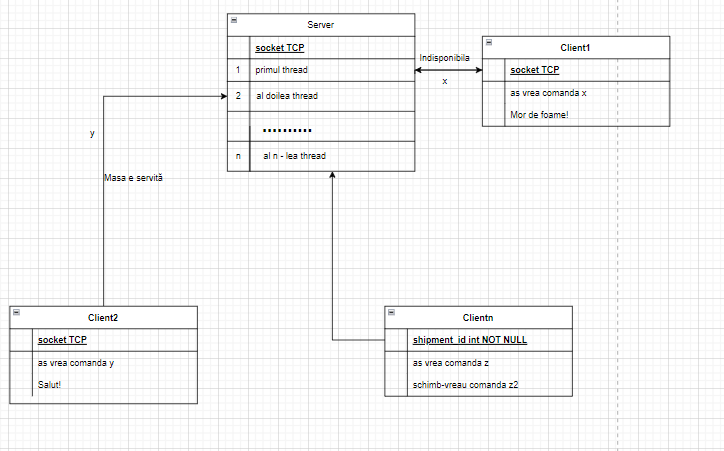
\includegraphics{diagrama.png}\\
- Serverul va face legătura cu clienți și va crea un thread pentru fiecare dintre clienti care se vor connecta in prime 20 secunde.Fiecare thread va fi indentificat printr-un id și va fi tratat de funcția treat.\\
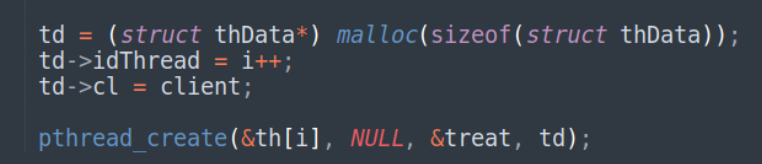
\includegraphics{cod1.png}\\Functia de treat va trata fiecare thread in parte, creând sctructurile de date și după va apela funția de comunicare, ea fiind apelată de fiecare thread.Funcția de comunicare va citi mesajul trimis de clientul respectiv și va crea un vector de adiacență pentru fiecare valoare(fiind maxim 5 feluri de mancare, indexurile vor fi de la 1 la 5). Vectorul fiind comun pentru toate threaduri incrementarea elementelor acestuia va fi blocata mutex.\\
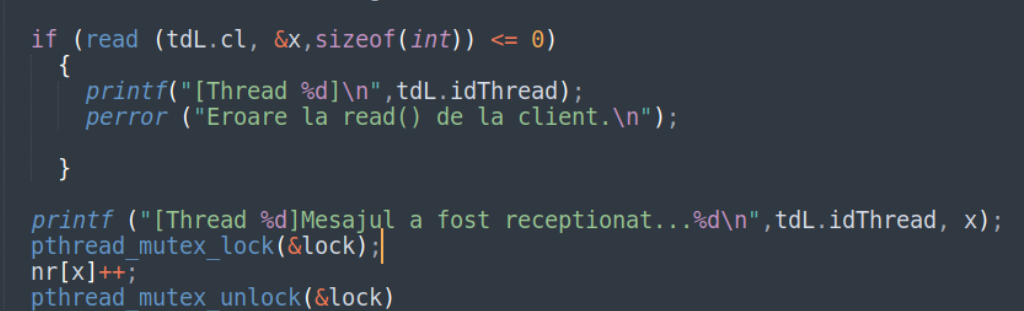
\includegraphics{cod2.png}\\Vectorul  nr este vectorul de adiacență și va fi incrementat în funcție de valorile citite din client în x. Vom apela functia sleep() pentru ca 
algoritmul să aiba timp să actualizeze valorile vectorului de adiacență și va răspunde clientului(respectiv idului threadului curent) conform valorii. Dacă valoarea curentă este egală cu valoare maximă a vectorului de adiacență  atunci serverul va trimite "Masa e servita", iar în caz contrar serverul va trimite "Indisponibil".\\ 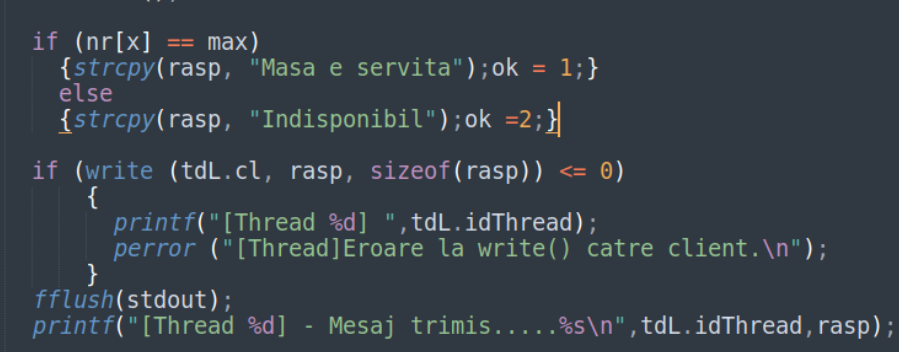
\includegraphics{cod3.png} \\Cazul indisponibil va face ca threadurile care au trimis acel mesaj să își reia execuția de la început(va citi din nou după ce va aștepta maxim 60 secunde, va recalcula vectorul de adiacență), reinițializând și vectorul de adiacență.După timerul de maxim 120s serverul nu va mai accepta clienți. Acest timer se va crea utilizând o variabilă clock\_t astfel că algoritmul în sine se va opri după acel interval lucrând doar threadurile. Programul va apela functia sleep de mai multe ori pentru a se asigura ca serverul prelucreaza in paralele informatiile, fara a avea scapari in cazul in care un client trimite comanda mai greu decat ceilalti\\
- Clientul va avea un algoritm mai simplu, el se va conecta la server la portul dat, și va trimite random un număr de la 1 la 5 reprezentând id-ul mâncărurilor posibile.Acest lucru va fi realizat prin funcțiile rand și srand() din $<$time.h$>$.\\ 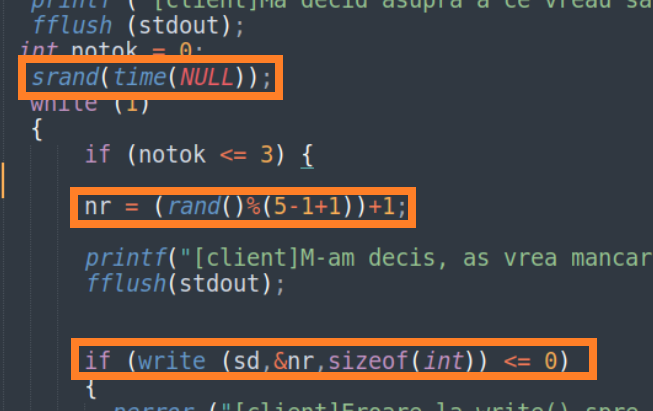
\includegraphics{cod4.png}\\ Apoi va primi răspunsul de la server,el putând fi "Masa e servita" sau "Indisponibil". În cazul indisponibil un counter va crește, iar când va ajunge la 3 va opri aplicația afișând  "Schimb cantina!Mor de foame!".În cazul contrar va afișa "Salut" și își va termina execuția.\\ 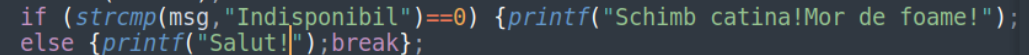
\includegraphics{cod5.png}\\

\section{Concluzii}
-Astfel algoritmul dat rezolvă problema dată ca input folosindu-se de un server concurent cu threaduri, fiecare thread calculând în paralel răspunsul pentru client.\\
- O posibilă îmbunătățire a soluție ar utiliza procese copil pentru fiecare client, în câte un file descriptor, utilizând funcția listen, procesele copil lucrând în paralel.
\section{Bibliografii}
- Cursul pentru Computer Networks - Informații despre comunicări, socketuri, threaduri.\\
- geeksforgeeks - mutex for linux thread-synchronization\\
- stackoverflow - David Guyon cod pentru a utiliza timer în c$\backslash$c++ utilizând clock.
\end{document}